\documentclass[12]{article}
\usepackage{listings}
\usepackage{color}
\usepackage{caption}
\definecolor{maroon}{rgb}{0.5,0,0}
\definecolor{darkgreen}{rgb}{0,0.5,0}
\definecolor{lightgray}{rgb}{0.95, 0.95, 0.95}
\definecolor{darkgray}{rgb}{0.4, 0.4, 0.4}
\definecolor{purple}{rgb}{0.65, 0.12, 0.82}

\lstdefinelanguage{CSS}{
    keywords={color,background-image,margin,padding,font,weight,display,position,top,left,right,bottom,list,style,border,size,white,space,min,width, transform, transition, transition-property, transition-duration, transition-timing-function},
    alsodigit={-},
    sensitive=true,
    morecomment=[l]{//},
    morecomment=[s]{/*}{*/},
    morestring=[b]',
    morestring=[b]"
}
\lstdefinelanguage{XML}
{
  basicstyle=\ttfamily,
  morestring=[s]{"}{"},
  morecomment=[s]{?}{?},
  morecomment=[s]{!--}{--},
  commentstyle=\color{darkgreen},
  moredelim=[s][\color{black}]{>}{<},
  moredelim=[s][\color{red}]{\ }{=},
  stringstyle=\color{blue},
  identifierstyle=\color{maroon}
}

\definecolor{javared}{rgb}{0.6,0,0} % for strings
\definecolor{javagreen}{rgb}{0.25,0.5,0.35} % comments
\definecolor{javapurple}{rgb}{0.5,0,0.35} % keywords
\definecolor{javadocblue}{rgb}{0.25,0.35,0.75} % javadoc
 
\lstset{language=Java,
basicstyle=\ttfamily,
keywordstyle=\color{javapurple}\bfseries,
stringstyle=\color{javared},
commentstyle=\color{javagreen},
morecomment=[s][\color{javadocblue}]{/**}{*/},
numbers=left,
numberstyle=\tiny\color{black},
numbersep=10pt,
tabsize=4,
showspaces=false,
showstringspaces=false}


\usepackage{subcaption}



\usepackage{Graphicx}

\usepackage{setspace}
\newcommand{\hsp}{\hspace{20pt}}
\newcommand{\HRule}{\rule{\linewidth}{0.5mm}}
\usepackage{minitoc}


\begin{document}
\onehalfspacing


\begin{titlepage}
  \begin{sffamily}
  \begin{center}

    
\includegraphics[scale=0.3]{C:/workplace/Java/project/inpt.png}~\\[1.5cm]

    \textsc{\LARGE Institut national des postes et télécommunications}\\[2cm]

    \textsc{\Large Rapport de projet}\\[1.5cm]

    % Title
    \HRule \\[0.4cm]
    { \huge \bfseries  Dynamic Web project :
    Psychologue enline \\[0.1cm] }

    \HRule \\[2cm]


    \begin{minipage}{0.4\textwidth}
      \begin{flushleft} \large
       Realisé par :\\
        Driouich Meryam\\
        Azzim Taha\\
      \end{flushleft}
    \end{minipage}
    \begin{minipage}{0.4\textwidth}
      \begin{flushright} \large
       Sous l'encadrement de :\\ \textbf{Dr Mahmoud Rlhamlaoui}
      \end{flushright}
    \end{minipage}

    \vfill

    % Bottom of the page
    {\large  Année universitaire :2020-2021}

  \end{center}
  \end{sffamily}
\end{titlepage}
\tableofcontents

\newpage

\section{Page Login}
\subsection{Page d'identification}
\indent

Créons premièrement un fichier Login.jsp dans lequel on aura la description de la page d'identification des différents utilisateurs.

\lstset{language=XML}
\begin{small}
\begin{lstlisting}
<!DOCTYPE html>
<html>
<head>
<meta charset="ISO-8859-1">
<title>Login</title>
</head>
<body>
<div align = "center"> 
 <form action="login" method="post">
  <table>
   <tr>
    <td align ="center">Nom d'utilisateur</td>
   </tr>
   <tr>
    <td><input type="text" name="nom"></td>
   </tr>
   <tr>
    <td align ="center">Mot de passe</td>
   </tr>
   <tr>
    <td><input type="password" nom="mot de passe"></td>
   </tr>
   <tr>
    <td align ="center"><input type="submit" value="Login"></td>
   </tr>
  </table>
 </form>
</div>
</body>
</html>
\end{lstlisting}
\end{small}
\newpage
On aura le resultat simple suivant\\

\begin{center}
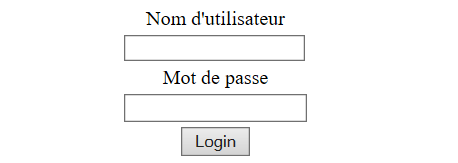
\includegraphics[scale=0.6]{C:/Workplace/java/project/1.png}
\captionof{figure}{Login.jsp}
\end{center}




\subsection{Connexion avec une base de données MySQL : vérification des identifiants}


\subsubsection{Classe Session}
On aura besoin d'une classe \textit{Session} (package : loginsesssion) qui va récupérer pendant chaque identification le nom et le mot de passe entrés.\\

\lstset{language=java}
\begin{lstlisting}

package loginsession;

public class session {
	private String nom;
	private String passe;
	public String returnNom() {
		return nom;
	}
	public String affecteNom(String nom) {
		this.nom = nom;
	}
	public String returnPasse() {
		return passe;
	}
	public String affectePasse(String passe) {
		this.passe = passe;
	}
}

\end{lstlisting}

\newpage
\subsubsection{Classe DB}

La classe DB (Package : base\_donnees) va permettre dans un premier lieux la connexion avec une base de données MySQL (userdb) qu'on va créer par la suite, puis vérifie si les identifiants (nom et mot de passe) entrés figurent dans cette base.\\
\lstset{language=java}
\begin{lstlisting}
package base_donnees;
import java.sql.Connection;
import java.sql.DriverManager;
import java.sql.PreparedStatement;
import java.sql.ResultSet;
import java.sql.SQLException;
import loginsession.*;
public class DB {
	private String dbUrl = "jdbc:mysql://localhost:3306/userdb?
                            useJDBCCompliantTimezoneShift=true&
                            useLegacyDatetimeCode=false&serverTimezone=UTC";
	private String dbUname = "AzzimDriouich";
	private String dbPassword = "0000";
	private String dbDriver = "com.mysql.cj.jdbc.Driver";
	public void loadDriver(String dbDriver)
	{
		try {
			Class.forName(dbDriver);
		} catch (ClassNotFoundException e) {
			e.printStackTrace();
		}
	}
	public Connection getConnection()
	{
		Connection con = null;
		try {
			con = DriverManager.getConnection(dbUrl, dbUname, dbPassword);
		} catch (SQLException e) {
			e.printStackTrace();
		}
		return con;
	}
	public boolean valider_donees(Session session)
	{
		boolean status = false;

		loadDriver(dbDriver);
		Connection con = getConnection();
		String sql = "SELECT * 
					  FROM login 
					  WHERE nom = ? 
					  AND mot_de_passe =?";
		PreparedStatement ps;
		try {
		ps = con.prepareStatement(sql);
		ps.setString(1, session.returnNom());
		ps.setString(2, session.returnPasse());
		ResultSet rs = ps.executeQuery();
		status = rs.next();
		
		} catch (SQLException e) {
			e.printStackTrace();
		}
		return status;
	}
}
\end{lstlisting}


\subsubsection{Création de la base de données "userdb"}


\begin{center}
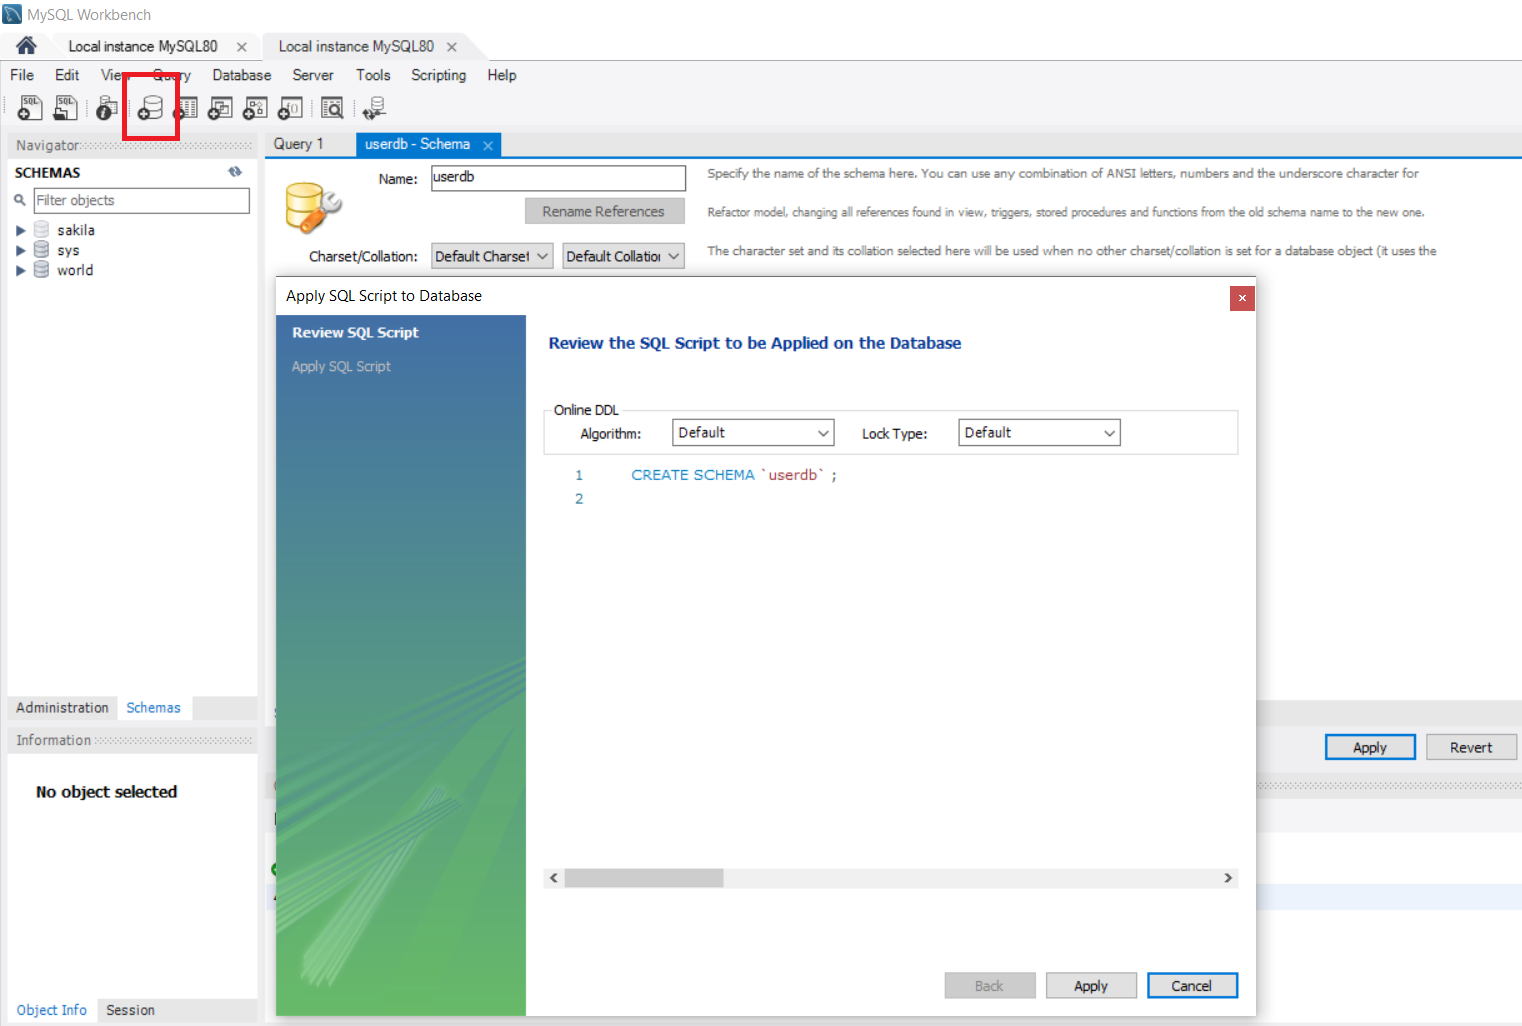
\includegraphics[scale=0.3]{C:/Workplace/java/project/2.png}
\captionof{figure}{create schema}
\end{center}

Après, on doit créer note tableau \textit{login} avec les deux colonnes \textit{nom} (Clé primaire et non null) et \textit{mot\_de\_passe} (non null).\\

\begin{center}
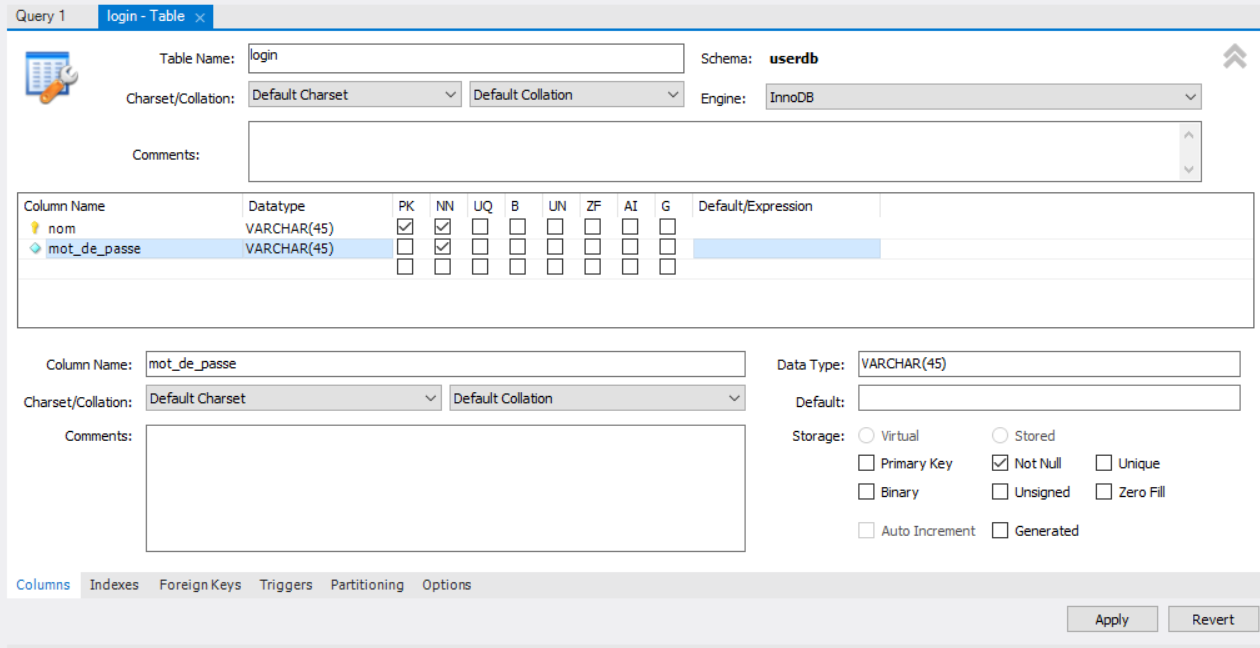
\includegraphics[scale=0.4]{C:/Workplace/java/project/3.png}
\captionof{figure}{Création de la table}
\end{center}

Afin de se connecter, on va insérer quelques utilisateurs à la table \textit{login}.\\


\begin{center}
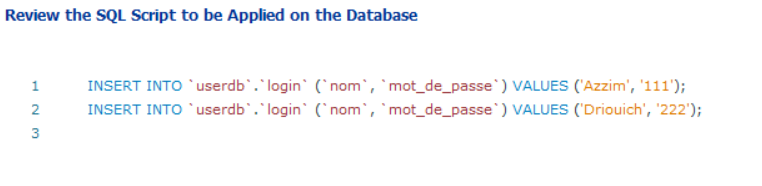
\includegraphics[scale=0.5]{C:/Workplace/java/project/4.png}
\captionof{figure}{Insertion des utilisateurs}
\end{center}






\subsection{Login servlet}

Dans le package web, introduisant la première servlet qui va se servir de l'authentification et diriger l'utilisateur vers sont compte si les identifiants sont corrects ou actualiser la page login sinon.\\

Pour cela, ajoutons un simple fichier Succes.jsp \\

\lstset{language=XML}
\begin{lstlisting}
<!DOCTYPE html>
<html>
<head>
<meta charset="ISO-8859-1">
<title>Succes</title>
</head>
<body>
Succes
</body>
</html>
\end{lstlisting}


\newpage

Puis la servlet serait comme suit :\\

\lstset{language=java}
\begin{lstlisting}
package web;

import java.io.IOException;
import javax.servlet.ServletException;
import javax.servlet.annotation.WebServlet;
import javax.servlet.http.HttpServlet;
import javax.servlet.http.HttpServletRequest;
import javax.servlet.http.HttpServletResponse;
import base_donnees.*;
import loginsession.*;

@WebServlet("/login")
public class LoginServlet extends HttpServlet {
	
	protected void doPost(HttpServletRequest request, 
						  HttpServletResponse response) 
	throws ServletException, IOException {
		String nom = request.getParameter("nom");
		String passe = request.getParameter("mot de passe");
		
	Session session = new Session();
	session.affecteNom(nom);
	session.affectePasse(passe);
	
	DB connexion_db = new DB();
	if(connexion_db.valider_donees(session)) {
		response.sendRedirect("Succes.jsp");
	}
	else {
		response.sendRedirect("login.jsp");
	}
	}
}

\end{lstlisting}



\subsection{Teste de login}

Exécutons le programme et essayons une authentification avec l'un des utilisateurs déclarés dans la base de données :\\

\begin{center}
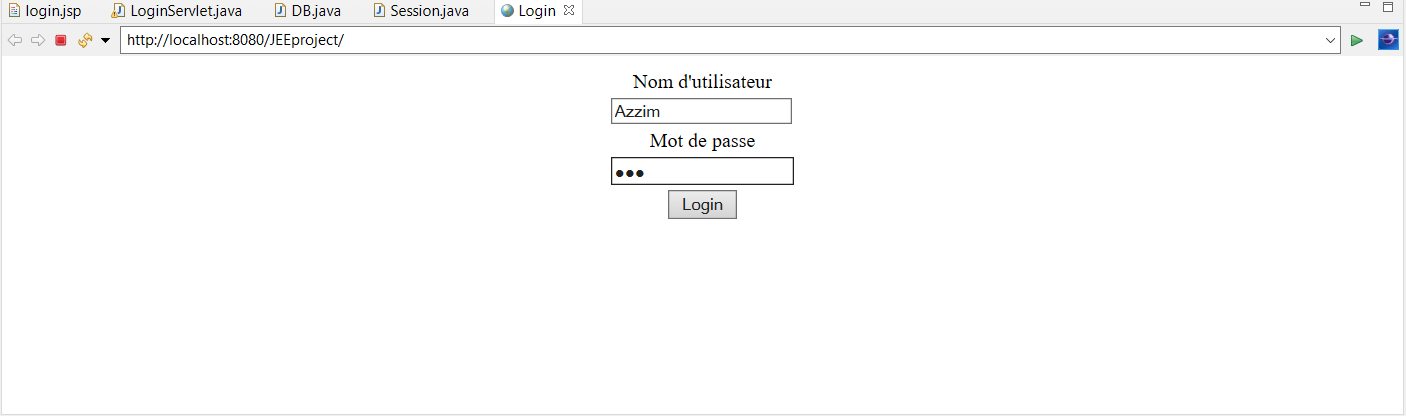
\includegraphics[scale=0.4]{C:/Workplace/java/project/5.png}
\captionof{figure}{Exécution}
\end{center}

\begin{center}
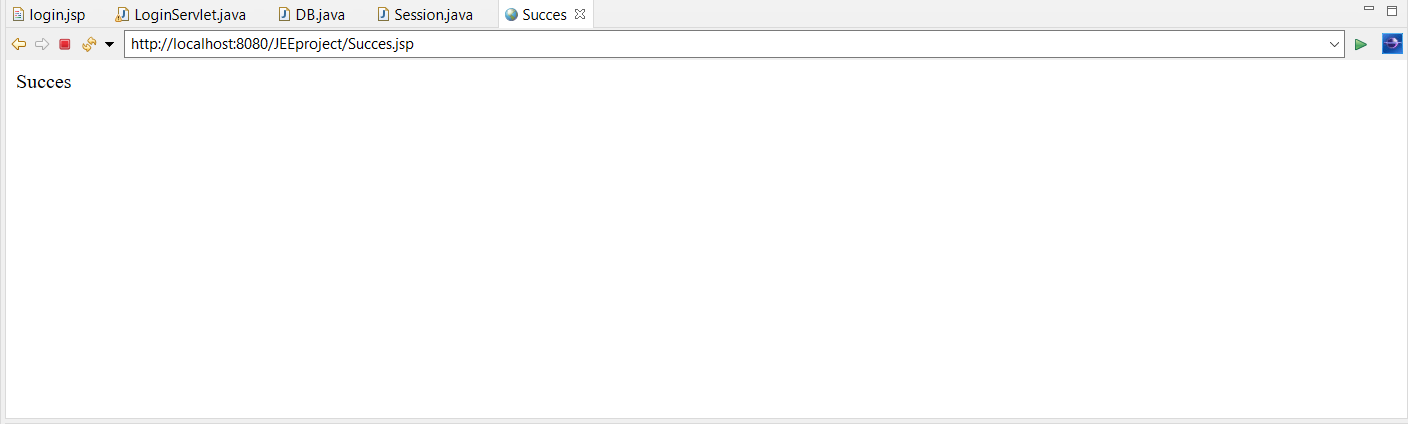
\includegraphics[scale=0.4]{C:/Workplace/java/project/6.png}
\captionof{figure}{Authentification avec succès}
\end{center}


\subsection{Configuration des differents acteurs : Psychologue, RH et Utilisateur }

Après l'authentification, l'inscrit doit être diriger vers sa page personnelle. On distingue entre 3 type d'inscrits : Psychologue, RH et utilisateur. De ce fait, on doit modifier la table \textit{login} en ajoutant la colonne \textit{type}.\\

\begin{center}
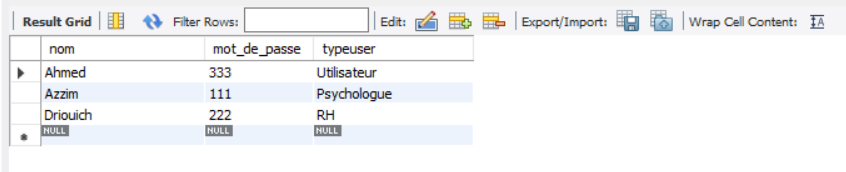
\includegraphics[scale=0.7]{C:/Workplace/java/project/7.png}
\captionof{figure}{Table login}
\end{center}

\newpage

Ensuite on doit modifier la classe \textit{Session} en ajoutant le String type et les méthodes affectType et returnType.\\

\lstset{language=java}
\begin{lstlisting}
package loginsession;

public class Session {
	private String nom;
	private String passe;
	private String typeUser;
	public void affectType(String typeUser) {
		this.typeUser = typeUser;
	}
	public String returnType() {
		return typeUser;
	}
	public String returnNom() {
		return nom;
	}
	public void affecteNom(String nom) {
		this.nom = nom;
	}
	public String returnPasse() {
		return passe;
	}
	public void affectePasse(String passe) {
		this.passe = passe;
	}
}

\end{lstlisting}

\newpage
Pour la classe DB, pendant la validation des identifiants (valide\_donnees), on récupère le type de l'inscrit et on affecte sa valeur à userType en faisant appel à affectType\\



\lstset{language=java}
\begin{lstlisting}
public boolean valider_donees(Session session)
{
	boolean status = false;

	loadDriver(dbDriver);
	Connection con = getConnection();
	String sql = "select * from login where nom =? and mot_de_passe =?";
	PreparedStatement ps;
	try {
	ps = con.prepareStatement(sql);
	ps.setString(1, session.returnNom());
	ps.setString(2, session.returnPasse());
	ResultSet rs = ps.executeQuery();
	status = rs.next();
	session.affectType(rs.getString("typeuser"));
	} catch (SQLException e) {
		e.printStackTrace();
	}
	return status;
}
\end{lstlisting}

\newpage

Finalement la servlet doit diriger chaque type d'inscrit vers sa page personnelle (Psychologue.jsp, RH.jsp ou Utilisateur.jsp)\\

\lstset{language=java}
\begin{lstlisting}
@WebServlet("/login")
public class LoginServlet extends HttpServlet {
	
	protected void doPost(HttpServletRequest request, 
						  HttpServletResponse response) 
	throws ServletException, IOException {
		String nom = request.getParameter("nom");
		String passe = request.getParameter("mot de passe");
		
	Session session = new Session();
	session.affecteNom(nom);
	session.affectePasse(passe);
	DB connexion_db = new DB();
	if(connexion_db.valider_donees(session)) {
		if(session.returnType().equals("Psychologue")) {
			response.sendRedirect("Psychologue.jsp");
		}
		else if(session.returnType().equals("Utilisateur")) {
			response.sendRedirect("Utilisateur.jsp");
		}
		else if(session.returnType().equals("RH")) {
			response.sendRedirect("RH.jsp");
		}
	}
	else {
		response.sendRedirect("login.jsp");
	}
	}

}
\end{lstlisting}


\subsection{Partie CSS}

Pour finir cette partie, introduisant un fichier css \textit{loginCSS.css} pour les raisons esthétiques.\\



\lstset{language=CSS}
\begin{lstlisting}
button {
  background-color: while;
  color: black;
  padding: 14px 20px;
  border-radius: 10px;
  margin: 8px 0;
  border: none;
  cursor: pointer;
  width: 100%;
}
input[type=text], input[type=password] {
  width: 100%;
  border-radius: 10px;
  padding: 12px 20px;
  margin: 8px 0;
  display: inline-block;
  border: 1px solid #ccc;
  box-sizing: border-box;
}
button:hover {
  opacity: 0.8;
  background-color: black;
  color: white;
}
body {
 background-image: url("1.gif");
 background-attachment: fixed;
 background-repeat: no-repeat;
 background-position: center;
 background-size: cover;
 background-color: white;
}

.login {
  overflow: hidden;
  opacity: 0.8;
  background-color: #8e8e8e;
  padding: 20px 30px 30px 30px;
  border-radius: 10px;
  top:100px;
  width: 400px;
  box-shadow: 5px 10px 10px rgba(green, 0.2);
}

\end{lstlisting}



le fichier \textit{login.jsp} sera aussi changé 


\lstset{language=XML}
\begin{small}
\begin{lstlisting}
<!DOCTYPE html>
<html>
<head>
<meta charset="ISO-8859-1">
<title>Login</title>
</head>
<link href="loginCSS.css" rel="stylesheet" type="text/css"><body>
<div align = "center">
 <form class = login action="login" method="post">
  <table>
   <tr>
    <td><input type="text" name="nom" placeholder="Nom d'utilisateur"></td>
   </tr>
   <tr>
    <td><input type="password" name="mot de passe" placeholder="Password"></td>
   </tr>
   <tr>
    <td align ="center"><button type="submit" value="Login">login</button></td>
   </tr>
  </table>
 </form>
</div>
</body>
</html>
\end{lstlisting}
\end{small}


Résultat final :

\begin{center}
\hspace*{-2cm}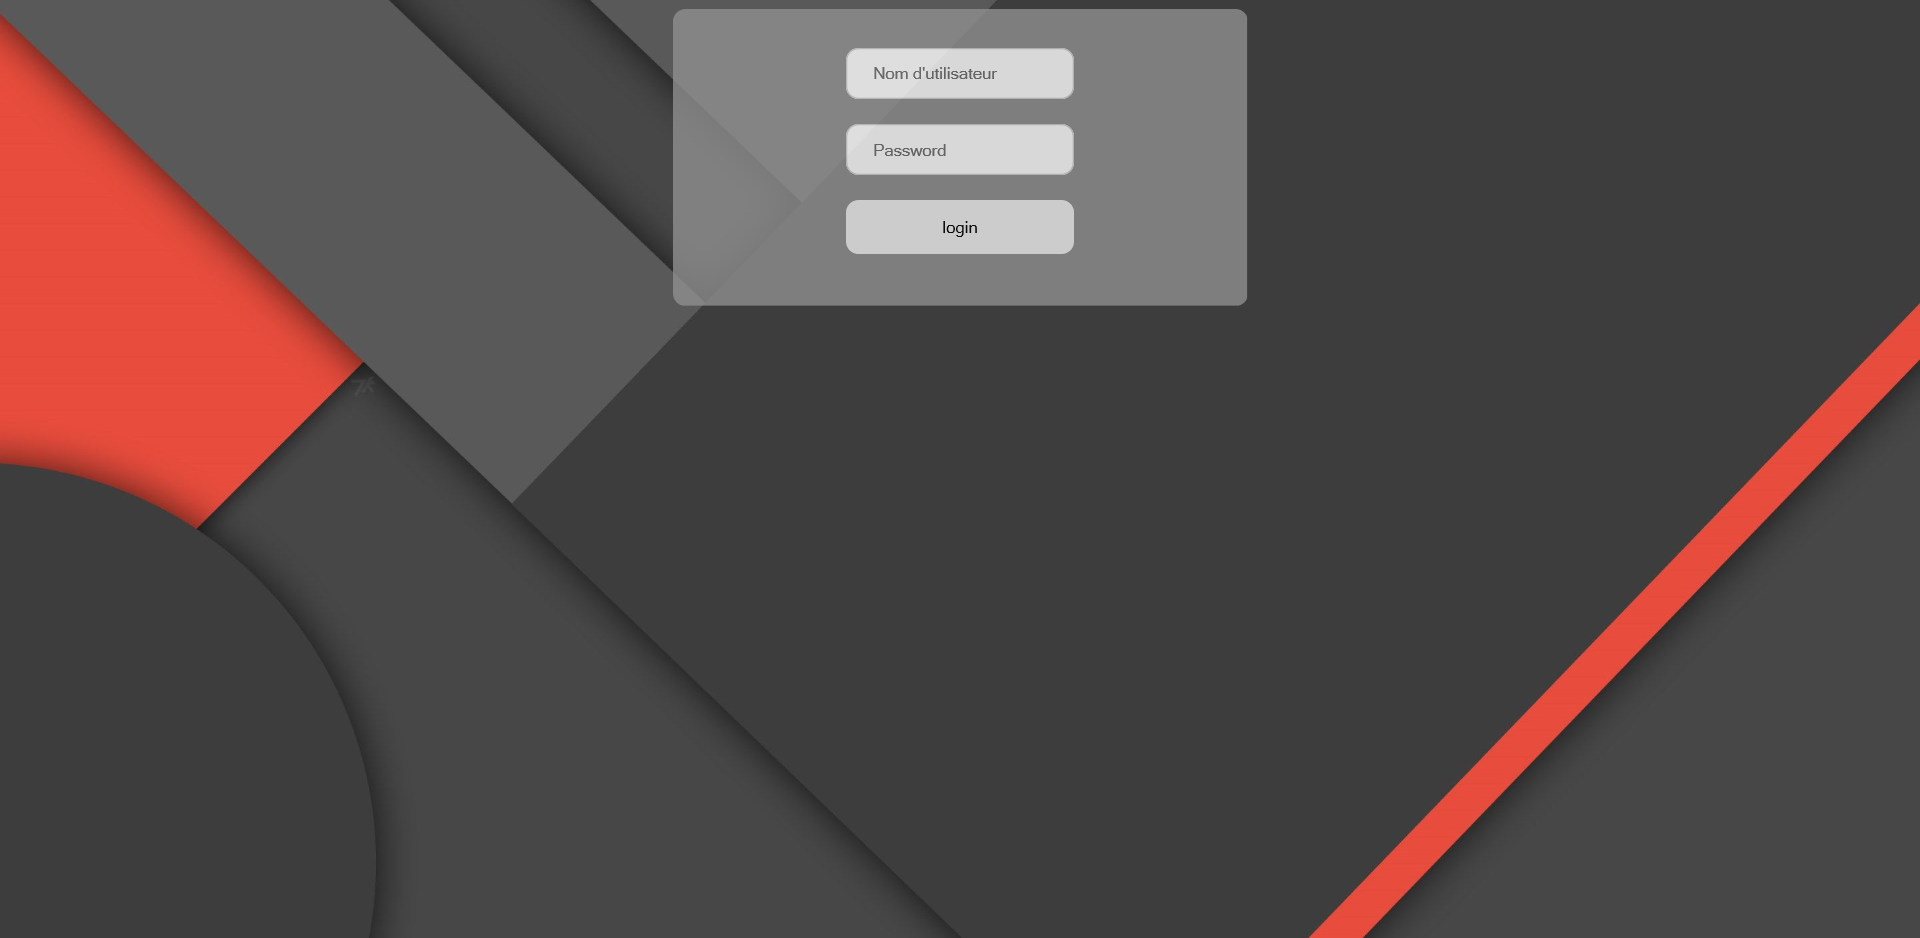
\includegraphics[scale=0.4]{C:/Workplace/java/project/14.png}
\captionof{figure}{Page login}
\end{center}














\section{Conception de la base de données}

De plus du tableau \textit{login} on aura besoin d'autres pour stocker les questions posés par les psychologues et les réponses récupérés de la part des utilisateurs.\\
On propose l'ajout de deux tableaux :\\
\begin{itemize}
\item Formulaires : renferme l'id du formulaire (Clé primaire), le nom du psychologue ( Créateur du formulaire ), le nom d'utilisateur ( Destinataire ) et l'état du formulaire ( Approuvé ou non par le RH ).\\
\item Questions : contient la question, son l'id ( Clé primaire ), l'id du formulaire où se trouve et les réponses fournies par les utilisateurs.
\end{itemize}


\begin{center}

\begin{tabular}{|c|c|c|c|}
\hline
\multicolumn{4}{|c|}{\textbf{Formulaires}}                                                                                                                                                                                                        \\ \hline
\textbf{id\_formulaire}                                    & \textbf{utilisateur}                                       & \textbf{psychologue}                                       & \textbf{etat}                                              \\ \hline
\textbf{\begin{tabular}[c]{@{}c@{}}.\\ .\\ .\end{tabular}} & \textbf{\begin{tabular}[c]{@{}c@{}}.\\ .\\ .\end{tabular}} & \textbf{\begin{tabular}[c]{@{}c@{}}.\\ .\\ .\end{tabular}} & \textbf{\begin{tabular}[c]{@{}c@{}}.\\ .\\ .\end{tabular}} \\ \hline
\end{tabular}



\begin{tabular}{|c|c|c|c|}
\hline
\multicolumn{4}{|c|}{\textbf{Questions}}                                                                                                                                                                                                          \\ \hline
\textbf{id\_question}                                      & \textbf{question}                                    & \textbf{id\_formulaire}                                          & \textbf{reponse}                                           \\ \hline
\textbf{\begin{tabular}[c]{@{}c@{}}.\\ .\\ .\end{tabular}} & \textbf{\begin{tabular}[c]{@{}c@{}}.\\ .\\ .\end{tabular}} & \textbf{\begin{tabular}[c]{@{}c@{}}.\\ .\\ .\end{tabular}} & \textbf{\begin{tabular}[c]{@{}c@{}}.\\ .\\ .\end{tabular}} \\ \hline
\end{tabular}
\end{center}


La création des deux tableaux consiste à lancer les deux requêtes :\\



\begin{center}
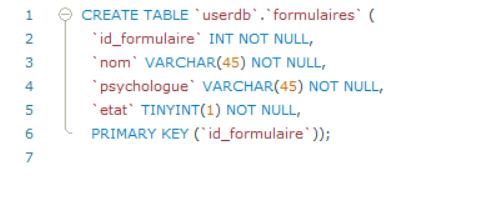
\includegraphics[scale=0.7]{C:/Workplace/java/project/15.png}
\captionof{figure}{table formulaires}

\vspace{1cm}
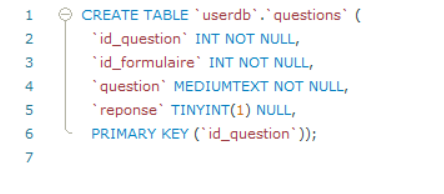
\includegraphics[scale=0.7]{C:/Workplace/java/project/16.png}
\captionof{figure}{table questions}
\end{center}

\textcolor{maroon}{NOTE : Pour éviter la confusion entre les id des formulaires et ceux des questions, les id des formulaires débuteraient toujours par un "10" (exemple : 101, 102 ...) alors que ceux des questions débuteraient avec un "20" (exemple : 201 202 ...)}\\


Insérant par suite quelques données dans les tables pour qu'elles nous aident pendant la construction des interfaces des utilisateurs (formulaire 101 avec 2 questions 201 et 202 et formulaire 102 avec une question 203)\\

 



\begin{center}
\hspace*{-2cm}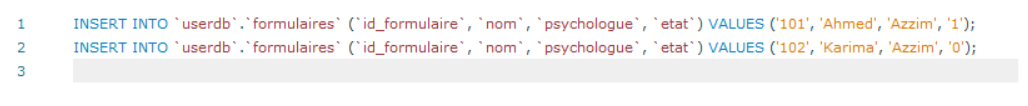
\includegraphics[scale=0.7]{C:/Workplace/java/project/17.png}
\captionof{figure}{table formulaires}

\vspace{1cm}
\hspace*{-3cm}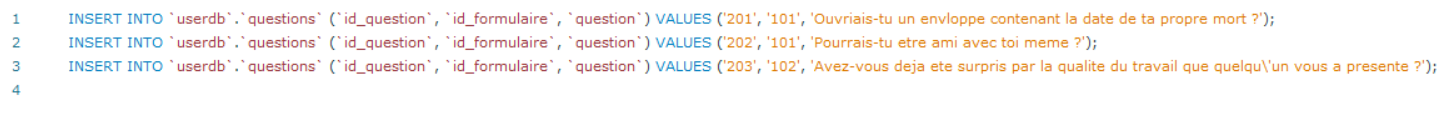
\includegraphics[scale=0.6]{C:/Workplace/java/project/18.png}
\captionof{figure}{table questions}
\end{center}


Maintenant que tout est prêt, construisons les interfaces des utilisateurs.\\

\section{Interface "Utilisateur"}
\indent


L'utilisateur doit être capable de voir les questions du formulaire fournit par le psychologue et approuvé par le RH. Il doit aussi avoir le droit de répondre à chaque question avec oui ou non. Finalement, il confirme ses réponses pour qu'elles soient envoyés au psychologue.\\
\subsection{Classe Question}

La première étape consiste à créer une classe \textit{Question} (Similaire à \textit{Session}) dont les attributs sont les colonnes du tableau Questions. \\





\lstset{language=java}
\begin{lstlisting}
package loginsession;

public class Question {
	public int id_question;
	public int id_formulaire;
	public String questiontext;
	public boolean reponse;
	
	public void affectIdQuestion(int id_question) {
		this.id_question =id_question;
	}
	public int returnIdQuestion() {
		return id_question;
	}
	public void affectIdFormulaire(int id_formulaire) {
		this.id_formulaire =id_formulaire;
	}
	public int returnIdformulaire() {
		return id_formulaire;
	}
	public String returnQuestion() {
		return questiontext;
	}
	public void affectQuestion(String questiontext) {
		this.questiontext = questiontext;
	}
	public boolean returnReponse() {
		return reponse;
	}
	public void affectReponse(boolean reponse) {
		this.reponse =reponse;
	}
	
}
\end{lstlisting}


\subsection{Chargement des questions depuis la base de données}

Ensuite, on déclare la fonction question\_utilisateur() qui prend en argument une \textit{Session} et une liste des objets de la classe \textit{Question} puis ajoute dans cette liste les questions du formulaire envoyé à cet utilisateur et qui sont approuvés par le RH.\\


Le tableau désiré est résultat de la requête :\\
\textbf{SELECT} * \\
\textbf{FROM} userdb.questions q \\
\textbf{INNER JOIN} userdb.formulaires f \\
\textbf{ON} f.id\_formulaire = q.id\_formulaire\\
\textbf{WHERE} f.nom=? \\
\textbf{AND} f.etat=1\\

Le champ f.nom serait remplis par session.nom.



\begin{small}
\lstset{language=java}
\begin{lstlisting}
public void question_utilisateur(Session session, List<Question> userquestion)
	{
		boolean status;

		loadDriver(dbDriver);
		Connection con = getConnection();
		String sql = "SELECT * FROM userdb.questions q 
					  INNER JOIN userdb.formulaires f 
					  ON f.id_formulaire=q.id_formulaire 
					  WHERE f.nom=? AND f.etat=1";
		PreparedStatement ps;
		try {
		ps = con.prepareStatement(sql);
		ps.setString(1, session.returnNom());
		ResultSet rs = ps.executeQuery();
		status = rs.next();
		while(status) {
			Question question = new Question();
			question.affectIdQuestion(rs.getInt("id_question"));
			question.affectIdFormulaire(rs.getInt("id_formulaire"));
			question.affectReponse(rs.getBoolean("reponse"));
			question.affectQuestion(rs.getString("question"));

			userquestion.add(question);
			status = rs.next();
		}
		} catch (SQLException e) {
			e.printStackTrace();
		}
	}
\end{lstlisting}

\end{small}



\subsection{Affichage des questions}

Finalement, dans la partie \emph{Utilisateur} de la servlet, on introduit la liste \textit{userquestion} des objets de la classe \textit{Question} qui serait remplies par la fonction \textit{question\_utilisateur()} et envoyée vers Utilisateur.jsp.


\begin{small}
\lstset{language=java}
\begin{lstlisting}
else if(session.returnType().equals("Utilisateur")) {
	List<Question> userquestion = new ArrayList<Question>();
	connexion_db.question_utilisateur(session, userquestion);
	request.setAttribute("userquestion", userquestion);
	request.setAttribute("utilisateur", session.returnNom());
	RequestDispatcher rst = request.getRequestDispatcher("Utilisateur.jsp");
	rst.forward(request, response);
		}
\end{lstlisting}

\end{small}


Finalement, la liste des questions peut être affichée à l'aide de foreach.\\

\begin{small}
\lstset{language=XML}
\begin{lstlisting}
<%@page contentType="text/html" pageEncoding="UTF-8"%>
<%@taglib uri="http://java.sun.com/jsp/jstl/core" prefix="c"%>
<!DOCTYPE html>
<html>
<head>
<meta charset="UTF-8">
<title>${utilisateur}</title>

</head>
<link href="UtilisateurCSS.css" rel="stylesheet" type="text/css">
<body>
 <form class=envoie action="envoie" method="post">
  <br>
  <br>
  <h1 align=center>Veuillez repondre aux questions suivantes</h1>
  <br>
  <br>
  <div class="container">
   <table align=center>
    <thead>
     <tr>
      <th>Question</th>
      <th>Reponse</th>
     </tr>
    </thead>
    <tbody>
     <c:forEach items="${userquestion}" var="question">
      <tr>
       <td><c:out value="${question.returnQuestion()}" /></td>
       <td>
        <select name="reponse" class="dropbtn">
         <option value="false">Oui</option>
         <option value="true">Non</option>
        </select></td>
      </tr>
     </c:forEach>
    </tbody>
    <thead>
     <tr>
      <td></td>
      <th align=center><button type="submit" value="Login">Envoyer</button></th>
     </tr>
    </thead>
   </table>
  </div>
 </form>
</body>
</html>
\end{lstlisting}

\end{small}


\subsection{Partie CSS}

Le fichier CSS décrivant la page utilisateur est donné par : 



\lstset{language=CSS}
\begin{lstlisting}
@import url(https://fonts.googleapis.com/css?family=Open+Sans:400,600);
h1{
	 font-size: 20px;
	 font-family: 'Courier New';
	 color : white;
}
button {
  background-color: white;
  color: black;
  display:inline-block;
  padding: 10px 30px;
  border-radius: 10px;
  font-size: 20px;
  margin: 30px 0;
  border: none;
  cursor: pointer;
  display: inline-block;
  transition: all 0.25s;
}

button:hover {
  opacity: 0.8;
  background-color: #E2B842;
  color: white;
}

*, *:before, *:after {
  margin: 0;
  padding: 0;
  box-sizing: border-box;
}
.dropbtn {
  background-color: #012B39;
  color: #ffffff;
  padding: 10px 30px;
  font-size: 15px;
  border: none;
  cursor: pointer;
}
body {
  background: #105469;
  font-family: 'Open Sans', sans-serif;
}
table {
  width: 70%;
  background: #012B39;
  border-radius: 0.25em;
  border-collapse: collapse;
  margin: 1em;
}
th {
  border-bottom: 1px solid #364043;
  color: #E2B842;
  font-size: 20px;
  font-weight: 600;
  padding: 0.5em 1em;
  text-align: Left;
}
td {
  color: #fff;
  font-weight: 400;
  padding: 0.65em 1em;
}
.disabled td {
  color: #4F5F64;
}
tbody tr {
  transition: background 0.25s ease;
}
tbody tr:hover {
  background: #014055;
}
\end{lstlisting}


Résultat donné pour utilisateur "Ahmed" :\\

\begin{center}
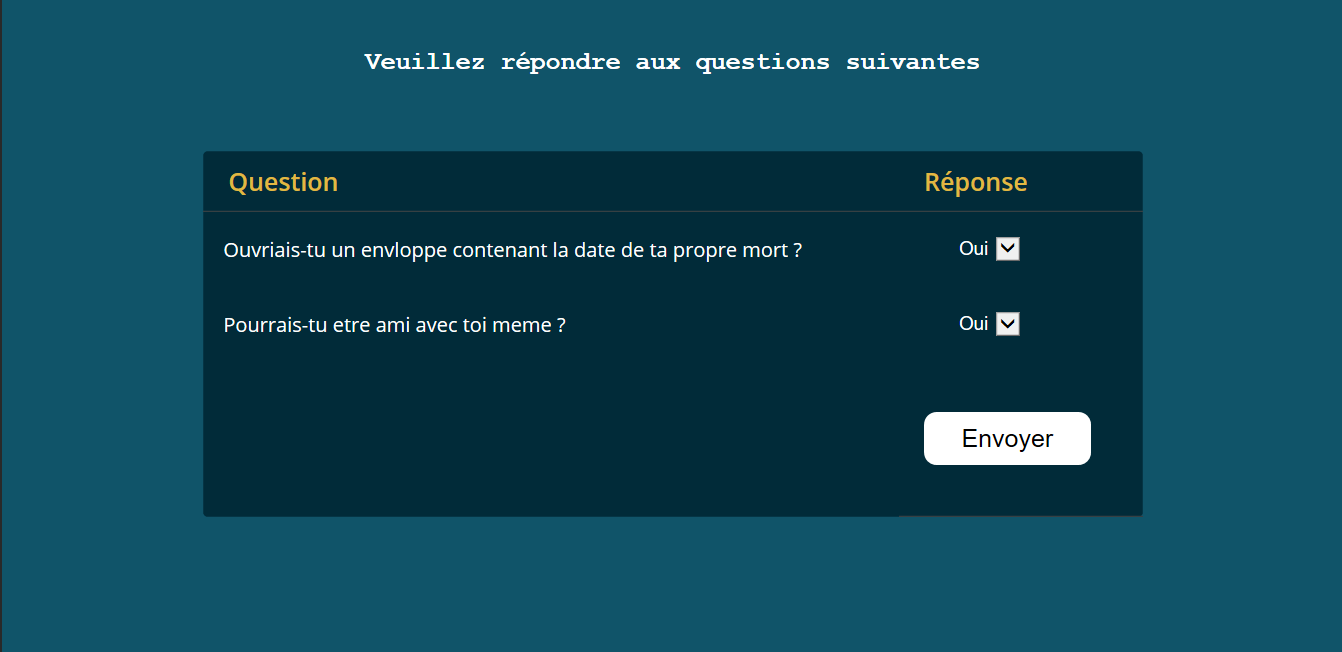
\includegraphics[scale=0.5]{C:/Workplace/java/project/19.png}
\captionof{figure}{Interface utilisateur}
\end{center}




































\end{document}